\chapter{Introduction}
\label{chap:introduction}

\section{Initial Situation}
Digital Twins (DT) are a key technology at the front of the fourth industrial revolution, coined Industry 4.0.
The latter term is characterized by the interaction of cyber-physical systems (CPS), the Internet of Things (IoT), and cloud computing to create smart factories with the goal of automation and efficiency \parencite{Oztemel2020}. Companies pursue this ideal by trying to remain competitive through the adoption of innovative technologies that promise enhanced productivity and reduced operational costs. One such technology promising this is the DT. It can be defined as a virtual representation of physical assets enabling real-time monitoring and optimization \parencite{Tao2018ijamt}. The DT bridges the connection between the two entities with a bi-directional data flow to exchange information and to influence the behaviour of the physical asset \parencite{grieves2014digital}. This technology in Industry 4.0 connects the physical and digital worlds through real-time data integration, simulation, and optimization \parencite{judijanto2024trends}.

Although this field is rapidly evolving, a common understanding of the definition of DT has yet to be established. The term was first introduced by Michael Grieves in 2002, defining it as a digital representation of a physical object or system \parencite{grieves2014digital}. However, the concept has evolved since then, encompassing a broader range of applications and technologies. Going back through the literature, there are three terms used to describe similar characteristics of DT: Digital Model (DM), Digital Shadow (DS), and Digital Twin (DT), see \Cref{fig:Kritzinger} \parencite{jones2020characterising,Zhang2021jmsy}.

\begin{figure}[htbp]
  \centering
  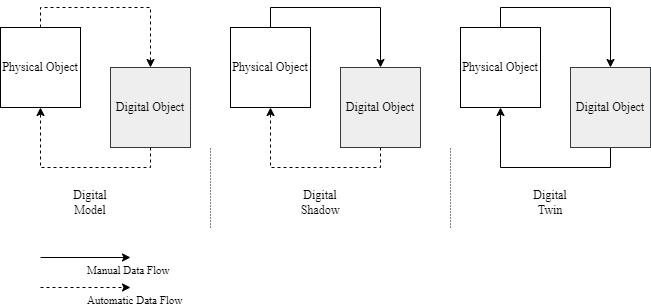
\includegraphics[width=0.8\textwidth]{figures/kritzinger.png}
  \caption{Comparison of Digital Shadow (DS), Digital Model (DM) and Digital Twin (DT) as presented by Kritzinger (2018). This distinction is crucial for understanding validation requirements across different digital representation types.}
  \label{fig:Kritzinger}
\end{figure}

The DM represents the most basic form. It contains manual data connections between physical and digital entities. These connections can be temporarily shifted or even disconnected. There is no control of the digital object over the physical entity. It rather is a simple or complex model \textit{describing} the modelled object. It can not make decisions by itself to influence the physical object. The reason lies in the potential outdated data the digital part possesses or in the fact that it does not contain logic to control the data flow back to the physical part by itself. The control and the obligation to interpret the results is completely in the hands of the modeller.
The DS is a more advanced version of the DM. It is a digital representation of the physical object, which is continuously updated with real-time data. The DS can be used for monitoring, analysis and simulation purposes. It can predict the future state of the physical object based on the current state and historical data. However, the DS is not able to influence the physical object. The control is, similar to the DM, still in the hands of the modeller. A DS is mainly used for simulation and in the literature often confusingly classified as a DT.
The DT is the most advanced version of the triplet. It is a digital representation of the physical object, which is also continuously updated with real-time data. The DT can be used for monitoring, analysis, and \textit{control} purposes. It can predict the future state of the physical object based on the current state and historical data. The DT can also influence the physical object by sending control signals to it. The control is partially or completely in the hands of the DT. The DT thus \textit{can} serve more purpose than modelling or simulating the physical object. It may serve as an autonomic system, updating itself or by help of the modeller \parencite{kritzinger2018digital}.

Digital twins are applied across various sectors, including manufacturing, defense, automotive, and recycling. This thesis focuses on manufacturing, particularly discrete material flow systems (DMFS). These systems process discrete objects (parts) that move along transportation routes or conveyor lines—either at regular or irregular intervals—integrating both production and logistics operations \parencite{arnold2005materialfluss, schwede2024learning}. A core simplification in their modeling is the abstraction of material flow as a sequence of discrete events, similar with the principles of discrete-event simulation (DES) \parencite{kovacs2016mathematical, robinson2014simulation}. DES is particularly well-suited for analyzing complex systems where state changes occur at discrete points in time, such as arrivals, departures, and processing steps \parencite{robinson2014simulation}.

In hindsight, DM played a crucial role in the design, planning, and control of DMFS, primarily through applications such as material flow simulations, logistic assistance systems, and digital factory implementations \parencite{Thiede2013}. However, advancements in both DS and DT have enabled a revolution from isolated, usecase-specific models toward complete digital models that span the entire lifecycle of DMFS \parencite{Abdoune2023}. This transition is largely driven by the increasing demand for predictive capabilities by stakeholders and automated decision support in manufacturing systems, reflecting the cornerstones of Industry 4.0 \parencite{frank2019industry}.

In practice, the automated data transfer between the digital model and the physical system is of secondary importance for DMFS management. Unlike in time-critical applications, human decision-makers remain an integral part of the control loop, ensuring that real-time automation is not always necessary \parencite{schwede2024learning}. Consequently, for this thesis, digital simulations and digital twins will be treated as equivalent concepts.

Beyond merely replicating the current state and managing historical data, digital twins serve a crucial function in predicting system behavior and evaluating potential modifications. The widespread adoption of DES within digital twins highlights the central role of simulation-based digital twins (SBDT) in DMFS \parencite{Lugaresi2021aifac}. As \citeauthor{schwede2024learning} emphasize, SBDTs provide decision support for optimizing cost and performance in highly competitive manufacturing environments. While current SBDTs are primarily developed and updated manually by domain experts, emerging research explores how machine learning (ML) can enhance predictive accuracy and automate model updates by automatically learning model characteristics, reducing costs and development time from data.

Thus, the progression from digital models to simulation-based digital twins reflects an ongoing shift towards data-driven, predictive, and increasingly automated representations of DMFS, ensuring more informed decision-making throughout the whole system lifecycle \parencite{boschert2016digital,lim2020state}.

\section{Problem}
Despite the immense transformative potential of DT, their implementation comes with significant challenges. The creation and maintenance of accurate Digital Twins require substantial investments in technology and domain knowledge. This investment yields no return if the resulting model fails to accurately represent the modelled entity or delivers incorrect results. Automatic generation may be an elegant solution, but posesses the risk of learning edge cases, ignoring the main trend. Manufacturing data used as training data must be preprocessed and cleaned thoroughly. The DT per definition has to be able to perform real time decision making without time lags. This yields the requirement to extract, transform, clean and load (ETL process, \cite{vassiliadis2002conceptual}) data on the fly, performing inference fully in memory. All these hurdles happening daily are challenges to automatic learning \parencite{ribeiro2016should,zhao2024data}. As industries integrate DT into their production processes, establishing trust becomes fundamental as well \parencite{trauer2022digital,arrieta2020explainable}. To gain widespread acceptance, the technology must demonstrate accuracy, transparency, and cost-efficiency \parencite{Wright2020amse,Shao2023mfglet}. Without these qualities, organizations will likely fall back to familiar methods, potentially building resistance to technological advancement \parencite{lapointe2005multilevel}.

Even if the automatic learning of the DT was performed sucessfully, the question of its correctness, precision and robustness remains unanswered. These questions are solved by validation, verification and uncertainty quantification frameworks (VVUQ) \parencite{sel2025survey}. Ensuring the validity, reliability, and accuracy of a Digital Twin is critical, yet traditional V&V approaches rely heavily on manual expert involvement and case-specific reference values \parencite{Bitencourt2023,hua2022validation}. This creates inefficiencies, particularly in the context of automated DT generation, where such manual processes conflict with the goal of reducing development effort. \cite{hua2022validation} even argue that there are no state of the art VVUQ methods for Digital Twins. One hurdle to standardized VVUQ frameworks is the lack of a clear definition for validity and verification in the context of Digital Twins \parencite{Bitencourt2023}.

For discrete material flow systems, these challenges are even more stressing due to their processual nature and inherent stochastic elements. Manufacturing processes may fail due to anomalies, resource constraints or human error. VVUQ approaches have to anticipate these risks. When DT for these systems are generated automatically, conventional validation approaches become problematic, as they negate much of the efficiency gained through automation. This creates an apparent paradox: Automated Digital Twin generation reduces initial development effort but potentially increases subsequent validation complexity, mitigating efficiency gains through automation. State of the art VVUQ frameworks have to uphold the efficiency gains earned while ensuring validity and reliability of the Digital Twin.

\section{Objective of the Thesis}
% This section includes: Motivation, Relevance, Research Questions, and Hypotheses

The thesis thus addresses this paradox by developing a data-driven framework for automated VVUQ of automatically generated, simulation-based DT which have been learned from data. The focus lies on DMFS due to their practical relevance and dynamical, processual nature. The endeavor can further be concretized by the following research questions (RQ):

\begin{itemize}
  \item \textbf{RQ1:} How can automated validation and verification processes for digital twins be efficiently implemented?
  \item \textbf{RQ2:} Which data-driven approaches are best suited to identify discrepancies between simulated behavior and real operational data in discrete material flow systems?
  \item \textbf{RQ3:} To what extent does the developed framework improve the quality and reliability of digital twins compared to traditional V&V methods?
\end{itemize}

This thesis addresses these questions by proposing that object-centric event logs—the same data structures often used to generate DT in manufacturing—can serve as the foundation for an automated, use case-independent validation and verification framework. Such an approach would maintain the efficiency benefits of automated generation while ensuring the resulting Digital Twins meet necessary quality standards. The development and monitoring of situative reference values which can not be generalized across all DTs is a key aspect of this approach. The framework will be evaluated using a case study from the discrete material flow domain, providing empirical evidence of its effectiveness in improving model accuracy and efficiency.

% This section includes: Motivation, Relevance, Research Questions, and Hypotheses
% Content goes here

Das Hauptziel dieser Arbeit ist die Entwicklung eines datengetriebenen Frameworks zur automatisierten Verifikation und Validierung von digital generierten, simulationsbasierten digitalen Zwillingen. Der Fokus liegt dabei auf diskreten Materialflusssystemen, da diese aufgrund ihrer Komplexität und Dynamik besondere Herausforderungen hinsichtlich der Modellgenauigkeit und Prozesssynchronisation aufweisen.
\section{Structure of the Thesis and Methodological Approach}
% Content goes here


\section{Problem}

Trotz des hohen Potenzials digitaler Zwillinge treten in der Praxis zahlreiche Herausforderungen auf. Die automatisierte Erstellung simulationsbasierter Modelle birgt das Risiko, dass wesentliche Systemkomponenten oder Interaktionsmuster unzureichend erfasst werden. Dies führt zu Diskrepanzen zwischen dem digitalen Modell und dem realen System, was im schlimmsten Fall die Grundlage für fehlerhafte Simulationen und falsche betriebliche Entscheidungen bildet. Traditionelle Verifikations- und Validierungsprozesse (V\&V) basieren häufig auf manuellen Prüfungen, die angesichts der Komplexität und der Datenmengen in modernen Produktionssystemen nicht mehr effizient durchführbar sind \parencite{Kritzinger2018}.

Ein weiteres Problemfeld stellt die Integration von Echtzeitdaten in die Simulationsmodelle dar. Während historische Daten die Basis statischer Modelle bilden, erfordert die dynamische Anpassung digitaler Zwillinge die kontinuierliche Auswertung und Synchronisation aktueller Betriebsdaten. Dies führt zu Herausforderungen hinsichtlich der Datenkonsistenz, -qualität und -verarbeitung. Zudem fehlt es oft an standardisierten Bewertungsmetriken, die eine objektive Beurteilung der Modellgüte ermöglichen. Diese Probleme machen deutlich, dass herkömmliche V\&V-Methoden nicht ohne Weiteres auf automatisiert generierte, simulationsbasierte digitale Zwillinge übertragbar sind.

Insbesondere in diskreten Materialflusssystemen, in denen zahlreiche Prozessvariablen und Interaktionskomponenten eine Rolle spielen, erfordert die Sicherstellung der Modellgenauigkeit neue Ansätze. Es besteht daher dringender Forschungsbedarf, um datengetriebene und automatisierte V\&V-Methoden zu entwickeln, die den spezifischen Anforderungen solcher Systeme gerecht werden \parencite{Kritzinger2018, Uhlemann2017}.

\section{Objective of the Thesis}

Das Hauptziel dieser Arbeit ist die Entwicklung eines datengetriebenen Frameworks zur automatisierten Verifikation und Validierung von digital generierten, simulationsbasierten digitalen Zwillingen. Der Fokus liegt dabei auf diskreten Materialflusssystemen, da diese aufgrund ihrer Komplexität und Dynamik besondere Herausforderungen hinsichtlich der Modellgenauigkeit und Prozesssynchronisation aufweisen.

\subsection*{Motivation und Relevanz}

Die Motivation dieser Forschungsarbeit ergibt sich aus mehreren zentralen Aspekten:
\begin{itemize}
  \item \textbf{Effizienzsteigerung:} Durch den Einsatz automatisierter V\&V-Methoden können Modellabweichungen frühzeitig erkannt und behoben werden, was zu einer signifikanten Reduktion von Fehlerquellen und Optimierungspotenzialen in Produktionsprozessen führt.
  \item \textbf{Digitalisierung und Vernetzung:} Mit der zunehmenden Integration von IoT und Sensorik in Produktionsanlagen steigt die Verfügbarkeit von Echtzeitdaten, die in digitalen Zwillingen verarbeitet werden können. Ein zuverlässiges V\&V-Framework stellt sicher, dass diese Daten adäquat in die Modelle einfließen.
  \item \textbf{Wettbewerbsvorteile:} Unternehmen, die in der Lage sind, ihre digitalen Modelle präzise und effizient zu validieren, sichern sich langfristig Wettbewerbsvorteile in einem zunehmend globalisierten Marktumfeld \parencite{Grieves2014}.
\end{itemize}

\subsection*{Forschungsfragen und Hypothesen}

Die Arbeit fokussiert sich auf folgende Forschungsfragen:
\begin{itemize}
  \item Wie können automatisierte Prozesse zur Verifikation und Validierung von digital generierten, simulationsbasierten digitalen Zwillingen effizient implementiert werden?
  \item Welche datengetriebenen Ansätze eignen sich am besten, um Abweichungen zwischen simuliertem Verhalten und realen Betriebsdaten in diskreten Materialflusssystemen zu identifizieren?
  \item Inwieweit verbessert das entwickelte Framework die Qualität und Zuverlässigkeit der digitalen Zwillinge im Vergleich zu traditionellen V\&V-Methoden?
\end{itemize}

Es wird die Hypothese aufgestellt, dass ein integriertes, datengetriebenes V\&V-Framework signifikante Verbesserungen in der Modellgenauigkeit und Effizienz der Validierungsprozesse bewirken kann. Durch den Einsatz moderner Datenanalysen und maschineller Lernverfahren sollen systematische Abweichungen frühzeitig erkannt und Korrekturmaßnahmen automatisiert eingeleitet werden \parencite{Tao2018}.

\section{Structure of the Thesis und Methodological Approach}

Der Aufbau dieser Arbeit gliedert sich in mehrere Kapitel, die im Folgenden kurz vorgestellt werden:

\begin{itemize}
  \item \textbf{Kapitel \ref{chap:literature}:} Umfassende Literaturrecherche. In diesem Kapitel werden die theoretischen Grundlagen digitaler Zwillinge, bestehende Simulationsansätze und aktuelle V\&V-Methoden analysiert.
  \item \textbf{Kapitel \ref{chap:framework}:} Entwicklung des datengetriebenen Frameworks. Hier werden die konzeptionellen und architektonischen Entscheidungen, die Auswahl der Algorithmen und die Implementierungsdetails dargestellt.
  \item \textbf{Kapitel \ref{chap:caseStudy}:} Fallstudie. Anhand eines konkreten Beispiels aus dem Bereich der diskreten Materialflusssysteme wird das entwickelte Framework empirisch validiert.
  \item \textbf{Kapitel \ref{chap:evaluation}:} Evaluation. Die Ergebnisse der Fallstudie werden hinsichtlich Modellgenauigkeit, Prozesszeiten und Fehlerhäufigkeiten quantitativ und qualitativ ausgewertet.
  \item \textbf{Kapitel \ref{chap:conclusion}:} Zusammenfassung und Ausblick. Abschließend werden die wesentlichen Erkenntnisse zusammengefasst, Limitationen diskutiert und Perspektiven für zukünftige Forschungsarbeiten aufgezeigt.
\end{itemize}

Methodologisch basiert die Arbeit auf einem iterativen Entwicklungs- und Validierungsansatz, der sowohl qualitative als auch quantitative Methoden integriert. Zunächst erfolgt eine detaillierte Literaturrecherche, um den aktuellen Stand der Technik zu erfassen und bestehende Forschungslücken zu identifizieren. Aufbauend auf diesen Erkenntnissen wird das Framework in modularer Form entwickelt. Die einzelnen Module – etwa für Datenerfassung, -vorverarbeitung, Modellgenerierung sowie die automatisierte V\&V – werden zunächst unabhängig implementiert und anschließend in ein Gesamtsystem integriert.

Ein zentraler Bestandteil der methodischen Vorgehensweise ist die empirische Validierung des Frameworks durch eine praxisnahe Fallstudie. Hierbei werden reale Prozessdaten eines diskreten Materialflusssystems herangezogen, um die Simulationsergebnisse kontinuierlich mit den tatsächlichen Betriebsdaten abzugleichen. Die Evaluation erfolgt durch die Analyse quantitativer Metriken (z. B. Abweichungsmaße, Reaktionszeiten) und wird durch qualitative Analysen ergänzt, um systemische Fehlerquellen aufzudecken \parencite{Uhlemann2017}.

Die Implementierung moderner Softwaretechnologien und datengetriebener Ansätze, wie etwa maschinelles Lernen, soll dabei helfen, die Validierungsprozesse zu automatisieren und flexibel an veränderte Betriebsbedingungen anzupassen. Der iterative Entwicklungsprozess ermöglicht es, das Framework kontinuierlich zu optimieren und auf die spezifischen Anforderungen unterschiedlicher industrieller Anwendungen zuzuschneiden. So wird ein dynamisches Instrument geschaffen, das nicht nur den theoretischen Anforderungen genügt, sondern auch in der Praxis anwendbar ist \parencite{Tao2018, Kritzinger2018}.

Zusammenfassend bietet diese Arbeit einen innovativen Beitrag zur Weiterentwicklung digitaler Zwillinge in diskreten Materialflusssystemen. Durch die Kombination theoretischer Fundierung, moderner datengetriebener Methoden und empirischer Validierung wird ein Framework vorgestellt, das signifikante Verbesserungen in der Modellgenauigkeit und Effizienz von V\&V-Prozessen ermöglicht. Die erzielten Ergebnisse tragen dazu bei, die Zuverlässigkeit digitaler Zwillinge zu erhöhen und bieten zugleich wertvolle Ansätze für die zukünftige Entwicklung in einer zunehmend digitalisierten und vernetzten Produktionslandschaft.
